\documentclass[
    11pt,
    a4paper
]{article}

% =========================================================
% IDIOMA, CODIFICACIÓN Y TIPOGRAFÍA
% =========================================================

\usepackage[utf8]{inputenc}
\usepackage[T1]{fontenc}
\usepackage{csquotes}
\usepackage[french]{babel}
\usepackage{lmodern}

% =========================================================
% GEOMETRÍA DE LA PÁGINA
% =========================================================

\usepackage[
    top=2.5cm,
    bottom=2.5cm,
    left=2.8cm,
    right=2.8cm
]{geometry}

% =========================================================
% MATEMÁTICAS
% =========================================================

\usepackage{amsmath}
\usepackage{amssymb}
\usepackage{amsfonts}
\usepackage{mathtools}
\usepackage{bm}

% =========================================================
% UNIDADES Y NOTACIÓN CIENTÍFICA
% =========================================================

\usepackage{siunitx}

\sisetup{
    output-decimal-marker={,},
    separate-uncertainty=true,
    per-mode=symbol
}

% =========================================================
% FIGURAS
% =========================================================

\usepackage{graphicx}
\usepackage{float}
\usepackage{subcaption}
\usepackage{placeins}

% Carpeta compartida (misma para todas las etapas) donde Etapa_1.py y demas scripts
% guardan sus figuras -- ver PLOTS_DIR_PAPER en Etapa_1.py
\graphicspath{{../plots/}}

% =========================================================
% TABLAS
% =========================================================

\usepackage{booktabs}
\usepackage{tabularx}
\usepackage{array}
\usepackage{multirow}
\usepackage{longtable}

% =========================================================
% COLORES
% =========================================================

\usepackage{xcolor}

\definecolor{linkcolor}{RGB}{0,70,140}
\definecolor{citecolor}{RGB}{0,100,70}
\definecolor{urlcolor}{RGB}{120,40,120}

% =========================================================
% HIPERVÍNCULOS Y REFERENCIAS CRUZADAS
% =========================================================

\usepackage[
    colorlinks=true,
    linkcolor=linkcolor,
    citecolor=citecolor,
    urlcolor=urlcolor,
    bookmarksopen=true,
    bookmarksnumbered=true
]{hyperref}

\usepackage[nameinlink, noabbrev]{cleveref}

% Nombres utilizados por cleveref
\crefname{equation}{équation}{équations}
\Crefname{equation}{Équation}{Équations}

\crefname{figure}{figure}{figures}
\Crefname{figure}{Figure}{Figures}

\crefname{table}{tableau}{tableaux}
\Crefname{table}{Tableau}{Tableaux}

\crefname{section}{section}{sections}
\Crefname{section}{Section}{Sections}

\crefname{subsection}{sous-section}{sous-sections}
\Crefname{subsection}{Sous-section}{Sous-sections}

% =========================================================
% ENCABEZADOS Y PIES DE PÁGINA
% =========================================================

\usepackage{fancyhdr}

\pagestyle{fancy}
\fancyhf{}

\fancyhead[L]{Validation du modèle à profondeur de coupe constante (Étape 1)}
\fancyhead[R]{\thepage}
\setlength{\headheight}{14.2pt}

\renewcommand{\headrulewidth}{0.4pt}
\renewcommand{\footrulewidth}{0pt}

% =========================================================
% FORMATO DE TÍTULOS
% =========================================================

\usepackage{titlesec}

\titleformat{\section}
    {\Large\bfseries}
    {\thesection.}
    {0.5em}
    {}

\titleformat{\subsection}
    {\large\bfseries}
    {\thesubsection.}
    {0.5em}
    {}

% =========================================================
% ESPACIADO
% =========================================================

\usepackage{setspace}

\setstretch{1.15}
\setlength{\parindent}{0pt}
\setlength{\parskip}{0.6em}

% =========================================================
% BIBLIOGRAFÍA
% =========================================================

\usepackage[
    backend=biber,
    style=numeric,
    sorting=none
]{biblatex}

\addbibresource{references.bib}

% =========================================================
% MICROTIPOGRAFÍA
% =========================================================

\usepackage[patch=none]{microtype}

% =========================================================
% COMANDOS PERSONALIZADOS
% =========================================================

% Notation reprise telle quelle du chapitre "Fondements du chatter et de la
% stabilité" (a_p, a_p^{lim}, a_p^{lim,crit}, K_c, zeta, Omega) -- ne pas la
% redéfinir localement, afin de rester cohérent avec le reste du mémoire.
\newcommand{\ap}{a_p}
\newcommand{\aplim}{a_p^{\mathrm{lim}}}
\newcommand{\apcrit}{a_p^{\mathrm{lim,crit}}}
\newcommand{\dxlsize}{\Delta_{\mathrm{dxl}}}
\newcommand{\RMS}{\operatorname{RMS}}

% $\eta$ est introduit spécifiquement dans cette étape pour désigner le rapport
% a_p/a_p^{lim,crit} -- $\varepsilon$ (déphasage) et $\lambda$ (racines de
% l'équation caractéristique) étant déjà pris par ailleurs dans le mémoire.
\newcommand{\etacrit}{\eta_{\mathrm{crit,th\acute{e}o}}}
\newcommand{\etasim}{\eta_{\mathrm{crit,sim}}}

% =========================================================
% INFORMACIÓN DEL DOCUMENTO
% =========================================================

\title{
    \textbf{Vérification de la limite de stabilité prédite par le modèle à profondeur de coupe constante (Étape 1)}
}

\author{
    Enrique Mireles
}

\date{\today}

% =========================================================
% INICIO DEL DOCUMENTO
% =========================================================

\begin{document}

\maketitle

\begin{abstract}

Ce document vérifie que le modèle numérique à profondeur de coupe constante
-- une fois la dynamique structurelle activée et la taille de dexel
retenue à l'issue de l'Étape~0 -- prédit correctement la profondeur de coupe
limite de stabilité, en la comparant à la limite théorique
\(\apcrit\) obtenue analytiquement pour le mode structurel dominant, à une
vitesse de rotation fixée. Un balayage de \(\eta = \ap/\apcrit\) est simulé,
chaque cas étant classé stable ou instable à partir de la pente du logarithme
du \(\RMS\) glissant de la vitesse structurelle. Le rapport \(\etasim\) estimé
par cette procédure s'avère systématiquement inférieur ou proche de l'unité,
indiquant un modèle globalement conservateur~: avec le dexel retenu à
l'Étape~0, la limite simulée reste néanmoins proche de la limite théorique.
Cette étape constitue le point de départ de l'étude de sensibilité au
raffinement du modèle, poursuivie à l'Étape~2.

\end{abstract}

\tableofcontents

\newpage

\section{Introduction}
\label{sec-introduction}

L'Étape~0 a permis de retenir une taille de dexel \(\dxlsize\) garantissant
une force de coupe simulée numériquement convergée, dans un cadre purement
cinématique où la dynamique structurelle était désactivée. Cette convergence
de la force ne garantit cependant pas, à elle seule, que le modèle dynamique
complet -- une fois la structure vibrante réintroduite -- restitue
correctement la limite de stabilité prédite par la théorie classique des
lobes~: c'est précisément cette question que la présente étape adresse.

Avec le dexel retenu, la dynamique du système usinant est activée, et un
balayage de profondeur de coupe est simulé autour de la limite théorique
\(\apcrit\), à une vitesse de rotation fixée. Chaque simulation est classée
stable ou instable a posteriori, et le point de transition ainsi obtenu est
comparé à la valeur théorique. Cette vérification est un préalable
indispensable~: toute étude ultérieure de la sensibilité du modèle à sa
discrétisation (Étapes~2 et~3) suppose que le modèle, à discrétisation fixée,
prédit déjà correctement la limite de stabilité classique.

\section{Modèle académique et paramètres}
\label{sec-modele}

\subsection{Cas académique}
\label{sec-cas_academique}

Le cas simulé reprend la configuration de l'Étape~0~: une opération de
tournage à un seul degré de liberté (1DDL) par mode, à profondeur de passe
\(\ap\) constante, sur une pièce cylindrique de rayon extérieur constant. La
seule différence par rapport à l'Étape~0 est que la dynamique structurelle
-- désactivée à l'Étape~0 pour isoler la convergence géométrique -- est ici
activée, ce qui rend le système sensible à la régénération de l'épaisseur de
copeau et donc à l'apparition du chatter.

% TODO: confirmer si la structure du modele dynamique (fonction de transfert
% a deux modes, cf. sec-parametres) est celle deja presentee au chapitre
% "Fondements du chatter et de la stabilite", ou si elle doit etre reintroduite
% ici -- dependra de la position finale de ce contenu dans le manuscrit.

\subsection{Paramètres dynamiques et paramètres de coupe}
\label{sec-parametres}

La structure est représentée par un modèle à deux modes propres découplés,
selon la formulation de superposition modale déjà introduite~: chaque mode
\(i\) est caractérisé par une raideur modale \(k_i\), un amortissement réduit
\(\zeta_i\) et un angle directionnel \(\theta_i\). Les paramètres retenus
sont rassemblés au \cref{tab-parametres_modaux}.

\begin{table}[H]
    \centering
    \caption{Paramètres modaux et paramètre de coupe retenus pour l'Étape~1.}
    \label{tab-parametres_modaux}
    \begin{tabular}{lccc}
        \toprule
        Mode & \(f_i\) [Hz] & \(k_i\) [N/m] & \(\zeta_i\) \\
        \midrule
        1 & 250 & \(2,26\times10^{8}\) & 0,012 \\
        2 & 150 & \(2,13\times10^{8}\) & 0,010 \\
        \bottomrule
    \end{tabular}

    \vspace{0.5em}
    \(\theta_1 = 30\,^{\circ}\), \(\theta_2 = -45\,^{\circ}\)~;
    coefficient spécifique de coupe \(K_c = 1000\)~N/mm\(^2\)~;
    avance \(f_z = 0,05\)~mm/tour.
\end{table}

% TODO: preciser la provenance de ces valeurs modales (identification
% experimentale, choix arbitraire pour l'etude academique, ou heritees d'un
% cas de la litterature) -- non explicite dans le code source consulte.

\subsection{Vitesse de rotation étudiée et profondeur critique théorique}
\label{sec-vitesse_ap_crit}

Le mode à \SI{150}{Hz} constitue, au voisinage de la vitesse de rotation
retenue, le mode gouvernant la limite de stabilité~: c'est le creux de sa
famille de lobes qui définit la profondeur critique la plus contraignante à
cette vitesse, le mode à \SI{250}{Hz} restant nettement moins restrictif dans
cette plage (\cref{fig-stability_map}, panneau de gauche). La vitesse de
rotation étudiée, \(\Omega = \SI{12094}{tr/min}\), est choisie au voisinage
immédiat du minimum de ce creux, de sorte que la profondeur critique
théorique correspondante,

\begin{equation}
    \apcrit = 8,6052\times10^{-3}~\text{m},
    \label{eq-ap_crit_theo}
\end{equation}

approche la limite inconditionnelle de stabilité du mode à \SI{150}{Hz} au
sens de la relation déjà établie pour \(a_p^{\mathrm{lim,crit}}\)
% TODO: verifier/citer le numero d'equation exact du chapitre "Fondements du
% chatter et de la stabilite" une fois ce contenu integre au manuscrit.
. Cette valeur, calculée analytiquement à partir des paramètres du
\cref{tab-parametres_modaux}, sert de référence unique pour tout le balayage
décrit à la \cref{sec-methode}.

\section{Méthode~: balayage et critère de classification}
\label{sec-methode}

\subsection{Rapport \texorpdfstring{\(\eta\)}{eta} et balayage}
\label{sec-balayage}

Chaque cas simulé est repéré par le rapport adimensionnel

\begin{equation}
    \eta = \frac{\ap}{\apcrit},
    \label{eq-eta}
\end{equation}

de sorte que \(\eta = 1\) correspond exactement à la limite théorique. Le
balayage débute à \(\eta = 0,5\) (cas largement stable) et progresse par pas
successifs~; il n'est pas fixé a priori mais raffiné itérativement~: dès
qu'une première paire consécutive stable\(\to\)instable est identifiée, nous
resserrons le pas autour de cette paire jusqu'à ce que l'écart entre les deux
valeurs de \(\eta\) encadrant la transition soit inférieur ou égal à
\(0,01\)
% TODO: preciser si ce seuil de 0,01 doit etre presente comme "1 %" ou "2 %"
% dans le manuscrit final (formulation encore en suspens, cf. historia
% narrativa de cette etape).
. Le point milieu de la dernière paire ainsi obtenue définit le rapport
critique simulé,

\begin{equation}
    \etasim = \frac{\eta_{-} + \eta_{+}}{2},
    \label{eq-eta_crit_sim}
\end{equation}

où \(\eta_{-}\) et \(\eta_{+}\) désignent respectivement le dernier cas
classé stable et le premier cas classé instable de la paire retenue. La
profondeur de coupe critique simulée correspondante et l'erreur relative de
détection s'écrivent

\begin{equation}
    a_{p,\mathrm{crit,sim}} = \etasim \, \apcrit,
    \qquad
    e_{\eta} = \bigl|\etasim - 1\bigr| \times 100.
    \label{eq-erreur_eta}
\end{equation}

\subsection{Critère de classification stable/instable}
\label{sec-classification}

Pour chaque cas, la vitesse structurelle simulée est traitée par une fenêtre
glissante de largeur \(T_w = \SI{0.1}{s}\), après exclusion des premiers
\SI{0.15}{s} correspondant au régime transitoire d'engagement de l'outil. Une
droite est ajustée au logarithme décimal du \(\RMS\) glissant ainsi obtenu en
fonction du temps~; le signe de la pente de cette droite fournit le critère
de classification~: une pente positive indique une croissance de
l'amplitude vibratoire (cas instable), une pente négative ou nulle indique
une décroissance ou une stabilisation (cas stable). Ce critère, fondé
uniquement sur la tendance globale du \(\RMS\) et non sur un indicateur de
détection élaboré, est délibérément simple~: son seul rôle ici est de
localiser la transition stable/instable avec une précision suffisante pour
valider le modèle, non de comparer des indicateurs entre eux -- cette
comparaison fait l'objet d'étapes ultérieures du pipeline.

% TODO: les sections "Application des indicateurs de la litterature",
% "Application de l'indicateur propose" et "Comparaison entre indicateurs"
% prevues dans le squelette du chapitre "Validation academique a profondeur
% de coupe constante" du manuscrit ne sont PAS couvertes par cette etape --
% seul le critere simple de pente du RMS ci-dessus est utilise. Decision a
% confirmer au moment de l'integration : laisser ces sections vides en
% attendant les etapes concernees, ou les completer avec ce critere simple a
% titre provisoire.

\section{Résultats}
\label{sec-resultats}

\subsection{Séries temporelles superposées}
\label{sec-resultats_series}

\begin{figure}[H]
    \centering
    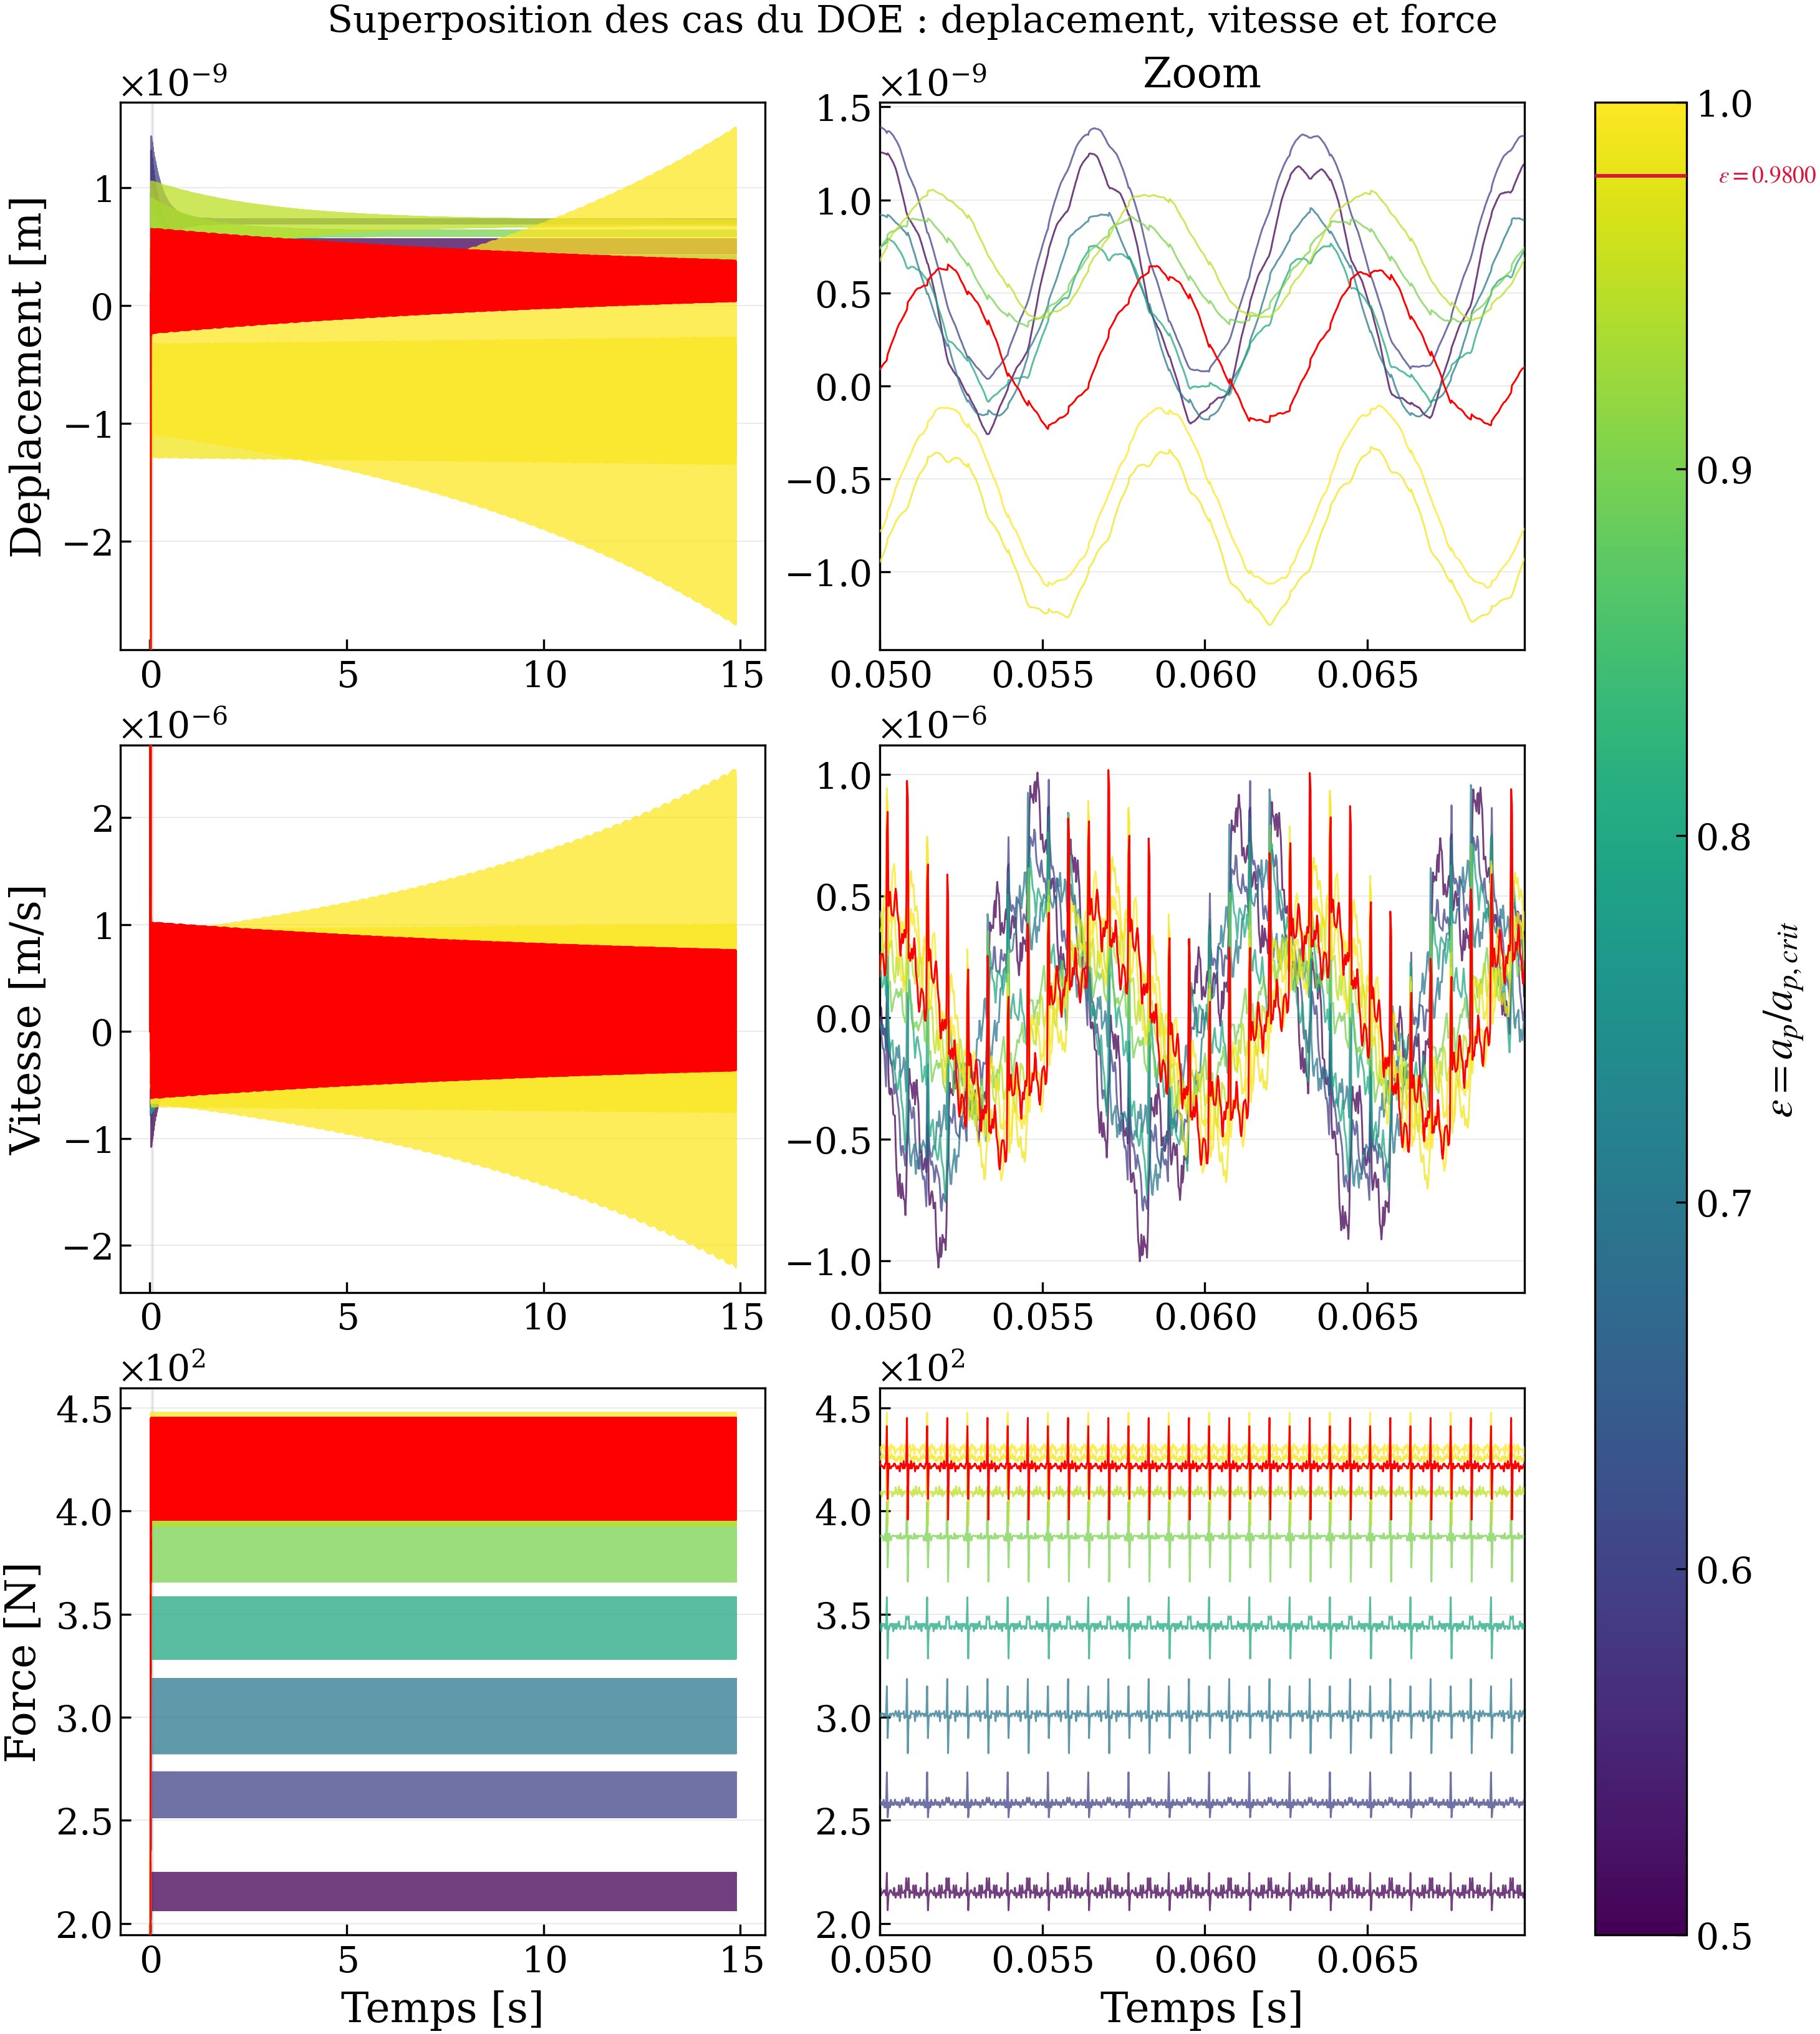
\includegraphics[width=\linewidth]{etapa1_fig_time_series_cases}
    \caption{Séries temporelles superposées de tous les cas du balayage en
    \(\eta\) (déplacement axial corrigé de la déflexion statique, vitesse
    axiale, effort de coupe), colorées selon \(\eta\) (échelle continue).
    Colonne de gauche~: signal complet, avec le transitoire initial exclu de
    l'échelle verticale. Colonne de droite~: zoom sur quelques révolutions en
    régime établi. Le dernier cas classé stable, correspondant à la borne
    inférieure de la transition retenue, est mis en évidence en rouge.}
    \label{fig-time_series_cases}
\end{figure}

Sur la \cref{fig-time_series_cases}, les cas à \(\eta\) faible présentent une
amplitude bornée, cohérente avec un régime stable, tandis que les cas à
\(\eta\) proche de ou supérieur à l'unité présentent une croissance continue
de l'amplitude sur la durée simulée, caractéristique du régime instable.
Le cas mis en évidence en rouge correspond au dernier cas encore classé
stable~: sa position, juste en deçà des cas dont l'amplitude diverge,
illustre visuellement la transition quantifiée à la
\cref{sec-resultats_lobes}.

\subsection{Diagramme de lobes et limite simulée}
\label{sec-resultats_lobes}

\begin{figure}[H]
    \centering
    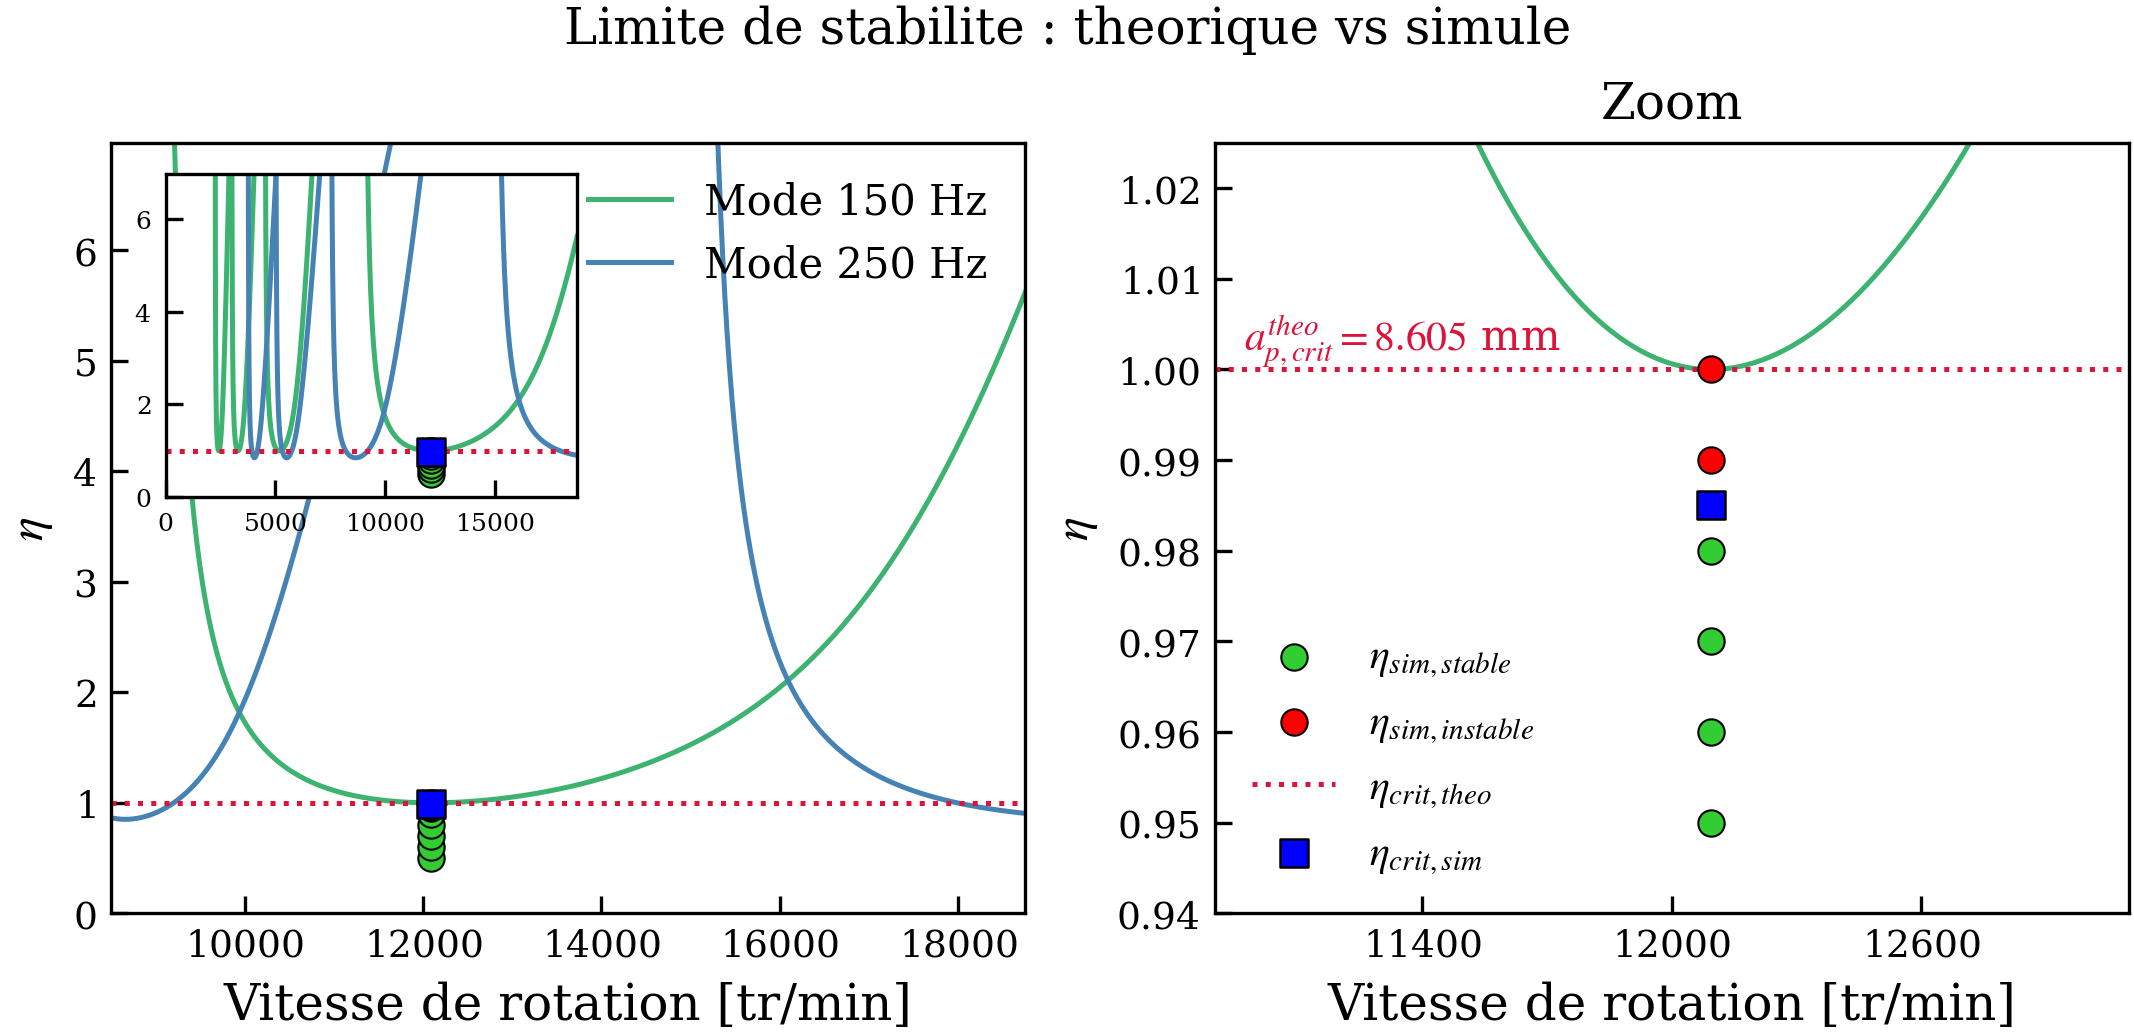
\includegraphics[width=\linewidth]{etapa1_fig_stability_map}
    \caption{Diagramme des lobes de stabilité (modes à \SI{150}{Hz} et
    \SI{250}{Hz}, calculés indépendamment l'un de l'autre) et cas du balayage
    en \(\eta\) reportés à la vitesse de rotation étudiée. Panneau de
    gauche~: vue d'ensemble, avec en médaillon le diagramme complet depuis
    une vitesse de rotation nulle. Panneau de droite~: zoom sur la zone de
    transition stable/instable, avec la profondeur critique théorique
    \(\apcrit\) annotée.}
    \label{fig-stability_map}
\end{figure}

Les deux modes de la \cref{fig-stability_map} sont calculés indépendamment
l'un de l'autre -- et non à partir d'une fonction de transfert combinée --
précisément pour que le creux de la famille de lobes du mode à \SI{150}{Hz}
touche exactement \(\eta = 1\) à la vitesse de rotation étudiée, par
construction de \(\apcrit\) à la \cref{sec-vitesse_ap_crit}~: une fonction de
transfert combinant les deux modes décale ce creux, les deux modes
interagissant dans le calcul du diagramme de lobes.
% TODO: cette independance des deux modes est une simplification de
% representation graphique -- confirmer si elle est physiquement justifiee
% dans le cadre de ce memoire (modes suffisamment separes en frequence pour
% negliger leur interaction) ou si elle doit etre signalee comme une
% limitation du diagramme presente.
Dans le panneau de droite, la transition simulée est encadrée par les
derniers cas classés stable et instable~; le rapport \(\etasim\) obtenu par
la \cref{eq-eta_crit_sim} se situe légèrement en deçà de l'unité, ce qui
correspond à une profondeur de coupe critique simulée légèrement inférieure à
la profondeur théorique \(\apcrit\).

\section{Discussion}
\label{sec-discussion}

Le rapport critique simulé \(\etasim\) obtenu est, de façon répétée à travers
les cas traités, inférieur ou très proche de l'unité~: le modèle tend donc à
être conservateur, c'est-à-dire à prédire l'apparition du chatter à une
profondeur de coupe légèrement inférieure à la profondeur théorique. Ce biais
n'est pas considéré comme un défaut rédhibitoire du modèle~; ce qui importe
pour la suite du travail est la précision de l'erreur de détection
\(e_{\eta}\), \cref{eq-erreur_eta}, plutôt que le signe de ce biais.

Avec la taille de dexel retenue à l'Étape~0, le modèle prédit correctement le
rapport \(\eta\) théorique, et un raffinement supplémentaire du dexel ne
modifie pas significativement ce résultat -- signe que la prédiction de la
limite de stabilité est, à cette taille de dexel, déjà convergée. À
l'inverse, avec un dexel plus grossier, le modèle sous-estime l'instabilité
(prédit plus de stabilité qu'il n'en existe réellement en théorie) --
comportement opposé à celui observé avec un dexel fin. La direction du biais
(conservateur ou optimiste) dépend donc de la taille de dexel employée~; ce
point est approfondi spécifiquement à l'Étape~2, où la taille de dexel est
balayée dans les mêmes conditions que la présente étude.

\section{Hypothèses et conditions de validité}
\label{sec-hypotheses}

\begin{itemize}
    \item La profondeur critique théorique \(\apcrit\) est calculée pour le
        mode à \SI{150}{Hz} seul~; elle suppose que ce mode reste le mode
        gouvernant sur toute la plage de \(\eta\) balayée, hypothèse
        cohérente avec la position de la vitesse de rotation étudiée au
        voisinage du creux de ce mode (\cref{sec-vitesse_ap_crit}).
    \item Le critère de classification stable/instable
        (\cref{sec-classification}) est un critère simple de tendance, non
        un indicateur de détection destiné à être comparé à d'autres~; il
        n'est utilisé ici que pour localiser la transition avec une
        précision suffisante à la validation du modèle.
    \item La taille de dexel employée est celle retenue à l'issue de
        l'Étape~0~; sa sensibilité propre sur la prédiction de \(\etasim\)
        n'est pas étudiée ici mais fait l'objet de l'Étape~2.
    \item Le raffinement itératif du balayage en \(\eta\)
        (\cref{sec-balayage}) suppose une transition monotone unique entre
        régime stable et régime instable~; il ne détecte pas d'éventuelles
        fenêtres de stabilité isolées à l'intérieur de la plage balayée.
\end{itemize}

\section{Conclusion}
\label{sec-conclusion}

Cette vérification constitue l'Étape~1 du pipeline~: avec la taille de dexel
retenue à l'Étape~0 et la dynamique structurelle activée, le modèle prédit
correctement la limite de stabilité théorique \(\apcrit\)
(\cref{eq-ap_crit_theo}), le rapport critique simulé \(\etasim\) obtenu par
la \cref{eq-eta_crit_sim} restant proche de l'unité
(\cref{fig-time_series_cases,fig-stability_map}). Cette validation ouvre la
voie à l'étude de sensibilité au raffinement spatial (Étape~2) puis temporel
(Étape~3) du modèle, dans les mêmes conditions que la présente étude.

% \printbibliography

\end{document}
